\subsection{\textit{Ad hoc on demand distance vector} - AODV}\label{subAODV}
O protocolo AODV \'e um protocolo reativo\cite{gorantala}, baseado em vetor de dist\^ancias, e pode ser considerado como uma combina\c{c}\~ao de outros dois protocolos, denominados DSR e DSDV. 
O AODV tem a base do DSR, o qual \'e baseado na forma de trabaho sob demanda, ou seja, descobre rotas somente quando necess\'ario, e utiliza os mecanismos de descoberta de rotas e manuten\c{c}\~ao de rotas.
Entretanto, o AODV utiliza a caracter\'istica do DSDV de obrigar todos os n\'os intermedi\'arios a estabelecerem dinamicamente entradas em tabelas de roteamento locais para cada destino ativo.
Cada n\'o tem conhecimento do pr\'oximo salto para alcan\c{c}ar o destino e a dist\^ancia em n\'umero de saltos.
Pode ser considerado como uma vers\~ao melhorada do DSDV, uma vez que seu funcionamento baseado em demanda minimiza o n\'umero de inunda\c{c}\~oes na rede exigido pelo DSDV para cria\c{c}\~ao de rotas.

\subsubsection{Processo de descoberta de rotas no AODV}
Quando um n\'o necessita encontrar uma rota para outro n\'o, e esta rota n\~ao est\'a presente na sua tabela de rotas, inicia um procedimento de descoberta de rotas (Figura \ref{figAodvRreq}), enviando pacotes \textit{Route Request} (RREQ) para todos os n\'os vizinhos, incluindo o \'ultimo n\'umero de sequ\^encia para aquele destino. 
Os pacotes RREQ s\~ao propagados pela rede at\'e alcan\c{c}ar o n\'o destino ou um n\'o intermedi\'ario com uma rota recente para o destino.

\begin{figure}[H]
	\centering
	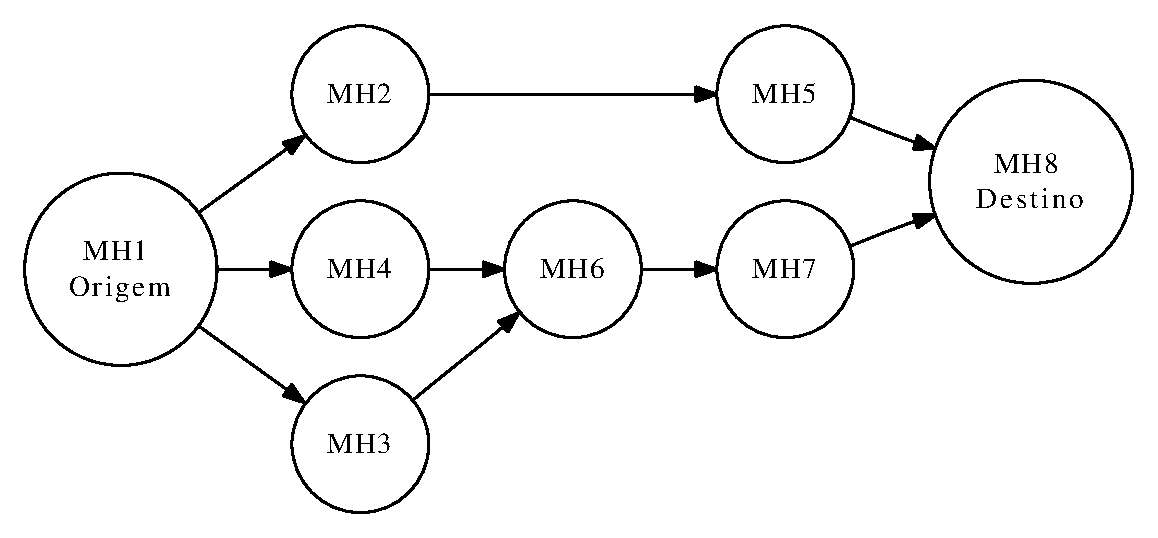
\includegraphics[scale=.5]{aodvRREQ.eps}
	\caption{Descoberta de rotas (RREQ) usando o protocolo AODV \cite{pereira}}
	\label{figAodvRreq}
\end{figure}

Durante o processo de encaminhamento do pacote RREQ, os n\'os intermedi\'arios gravam em suas tabelas de rotas o endere\c{c}o do vizinho que encaminhou o pacote. 
Desta forma, estabelece um caminho reverso que ser\'a utilizado pelo pacote \textit{Route Reply} (RREP) para alcan\c{c}ar o n\'o de origem (Figura \ref{figAodvRrep}), quando a rota para o destino for encontrada.

\begin{figure}[H]
	\centering
	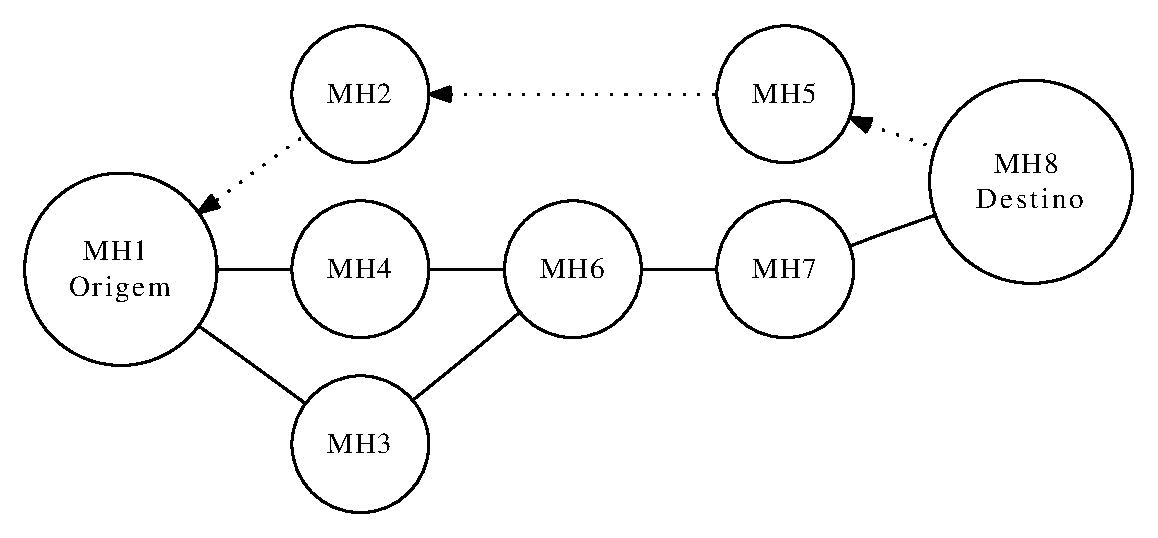
\includegraphics[scale=.5]{aodvRREP.eps}
	\caption{Propaga\c{c}\~ao do \textit{Route Reply} (RREP) no protocolo AODV \cite{pereira}}
	\label{figAodvRrep}
\end{figure}

Em cada tabela de roteamento \'e mantido o conjunto de n\'os antecessores que utilizam esta entrada para rotear pacotes de dados. Ent\~ao, quando uma conex\~ao \'e interrompida, estes n\'os antecessores s\~ao notificados com pacotes \textit{Route Error} (RERR). Cada n\'o antecessor encaminha este pacote para sua lista de n\'os antecessores, permitindo assim que efetivamente seja propagada a informa\c{c}\~ao de conex\~ao falha.

\begin{figure}[H]
	\centering
	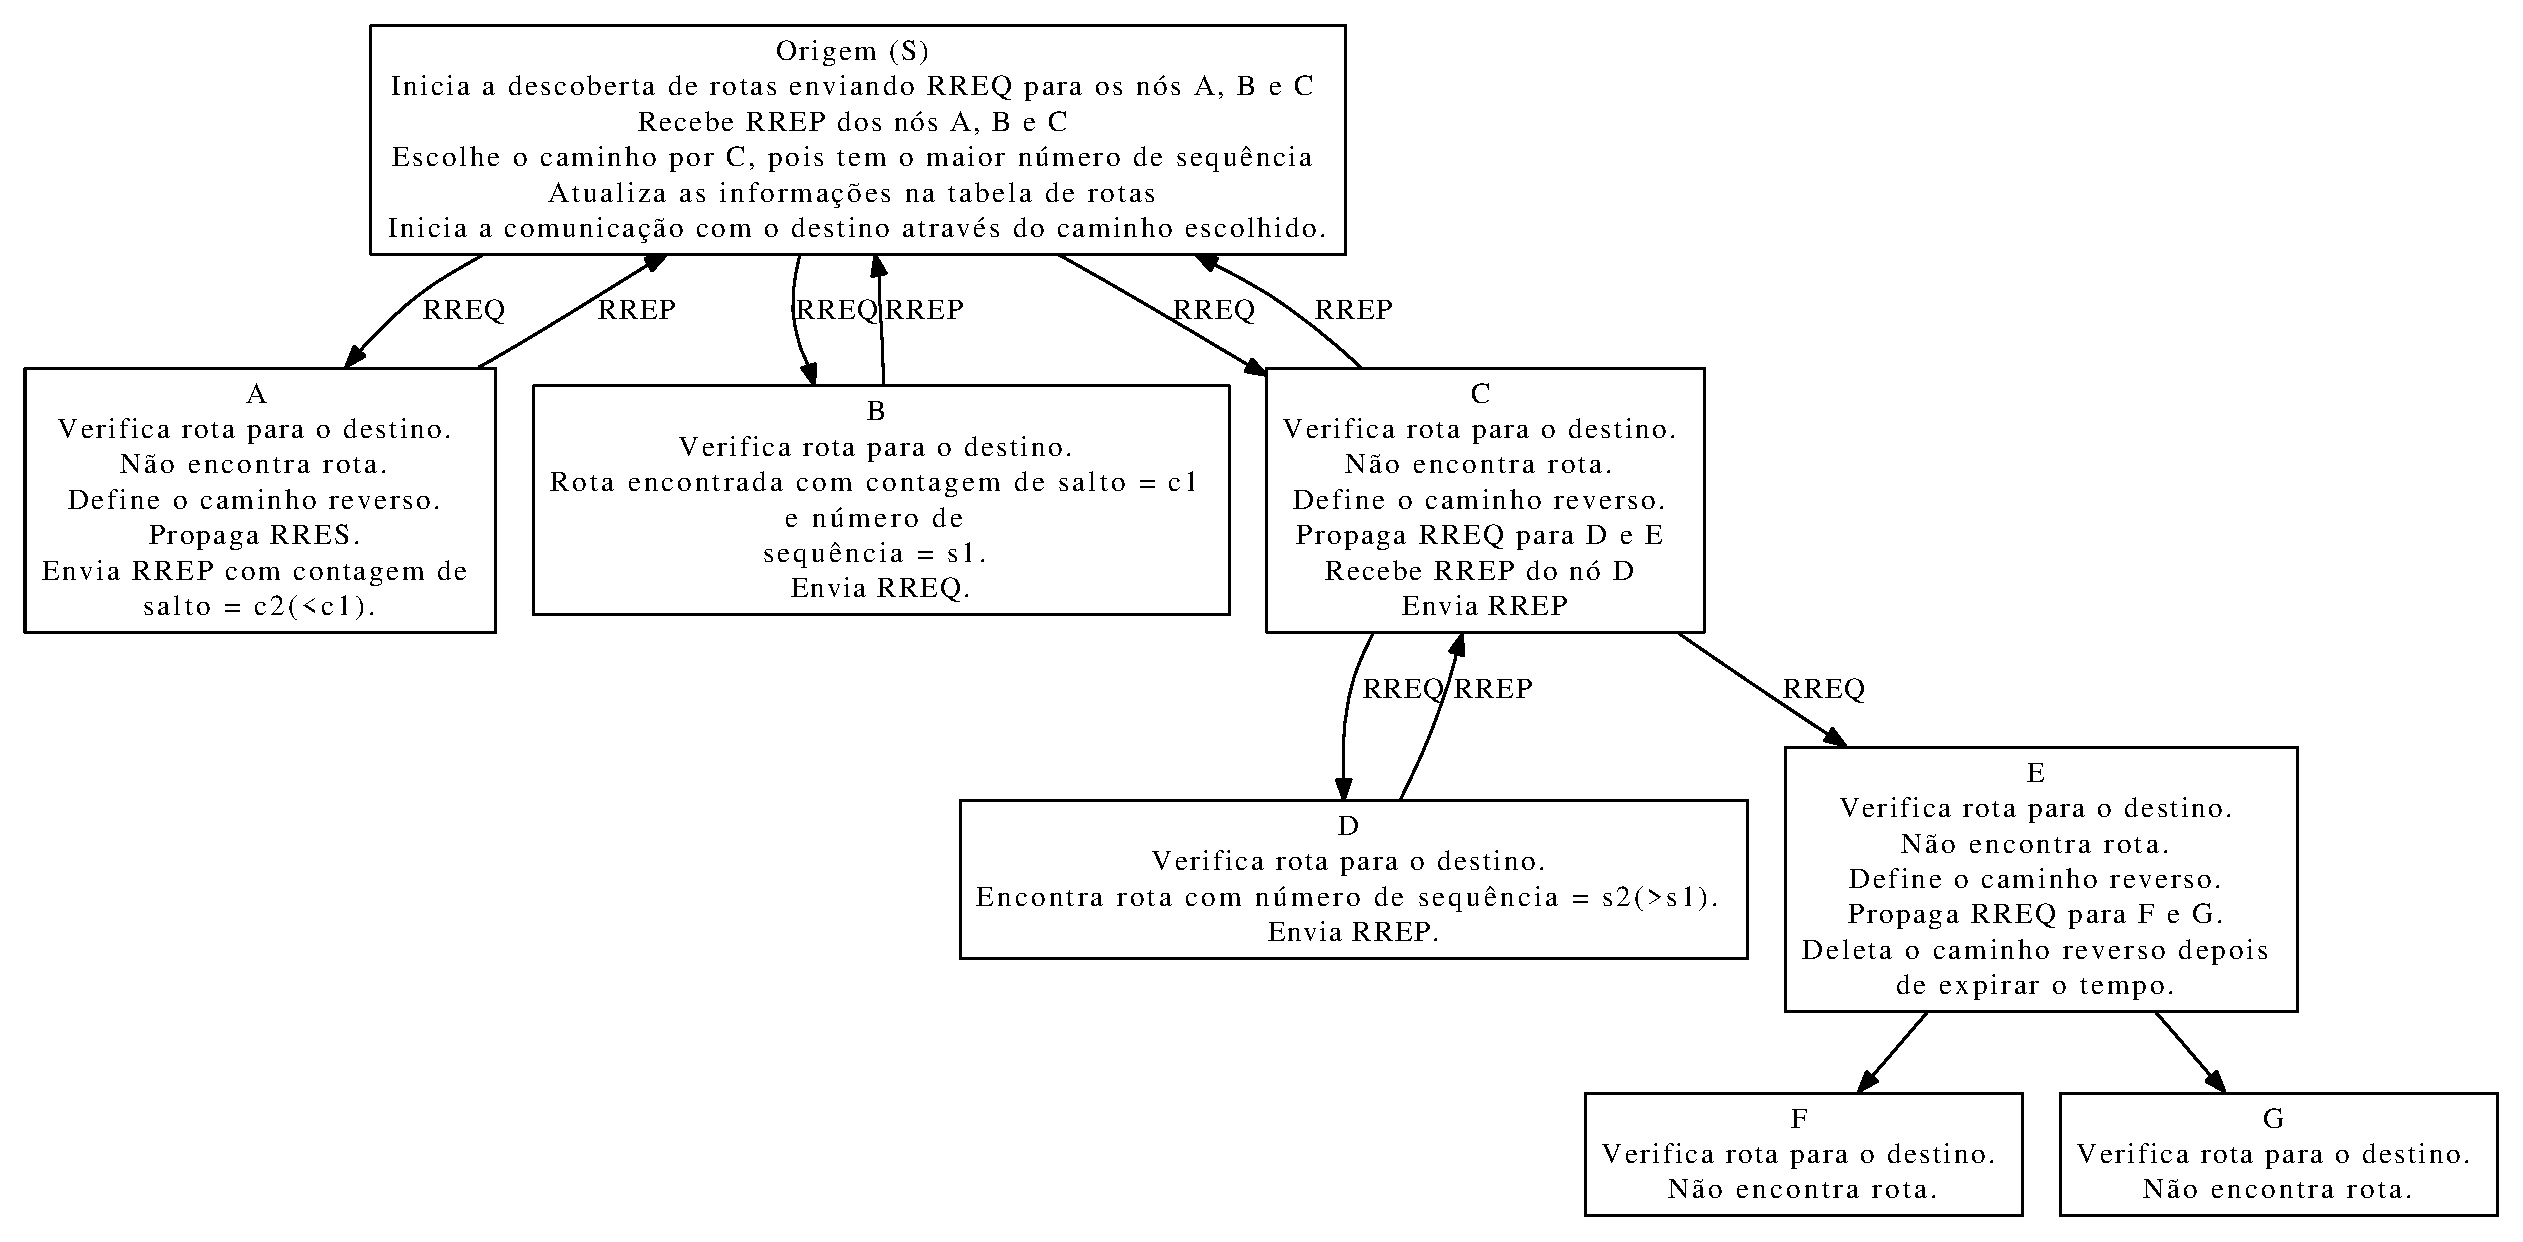
\includegraphics[scale=.43]{aodvOperation.eps}
	\caption{Processo de cria\c{c}\~ao de rotas no AODV \cite{gorantala}}
	\label{figOpAODV}
\end{figure}
Acima a Figura \ref{figOpAODV} \'e um exemplo de como o protocolo AODV encontra uma rota para um destino.
Segue passo-a-passo a explica\c{c}\~ao do processo exibido na Figura \ref{figOpAODV} acima.
\begin{enumerate}
	\item "Origem S" precisa enviar dados ao destino.
	\item "S" envia RREQ para seus vizinhos "A", "B" e "C".
	\item "B" encontra o caminho em sua tabela de roteamento (com n\'umero de sequ\^encia = s1 e contagem de salto = c1) e envia RREP para "S".
	\item "C" ativa caminho reverso.
	\item "C" redireciona RREQ para seus vizinhos "D" e "E".
	\item "E" ativa caminho reverso.
	\item "E" redireciona RREQ para seus vizinhos "F" e "G".
	\item "E" deleta o caminho reverso ap\'os um per\'iodo de tempo limite, uma vez que n\~ao recebe qualquer RREPs dos n\'os "F" e "G".
	\item "D" encontra o caminho para destn (com n\'umero de sequ\^encia = s2, o qual \'e maior que s1 e contagem de salto c1) em sua tabela de roteamento e envia RREP para "C".
	\item "C" recebe RREP de "D" e ativa o caminho de reencaminhamento e reencaminha RREP para "S".
	\item "A" define o caminho reverso; redireciona RREQ para seus vizinhos; recebe RREP (com caminho de contagem de saltos c2, o qual \'e maior que c1); define o caminho de redirecionamento; e redireciona o RREP para "S".
	\item "S" recebe uma inform\c{c}\~ao de caminho de "C" (o qual foi criado por "D"), dando prioridade ao caminho com o n\'umero de sequ\^encia maior e segunda prioridade com o caminho com a menor contagem de saltos. Apesar do caminho por "A" ter uma menor contagem de saltos, isso \'e ignorado, porque o n\'umero de sequ\^encia \'e maior para o caminho de "C".
\end{enumerate}

\subsubsection{Vantagens do AODV}
\begin{itemize}
	\item Por causa de sua natureza reativa, o AODV pode lidar com o comportamento di\^amico das redes \textit{ad hoc} \cite{schwingenschlogl}.
	\item Utilizado tanto para \textit{unicasts} quanto \textit{multicasts} com a \textit{flag} 'J'\footnote{\textit{Join in group} - Usado para aproveitar rota de outros n\'os.} nos pacotes \cite{ramachandranTech}.
\end{itemize}

\subsubsection{Limita\c{c}\~oes e desvantagens do AODV}
\begin{itemize}
	\item \textbf{Necessidade de um meio de propaga\c{c}\~ ao:} O algoritmo necessita que os n\'os no meio da propaga\c{c}\~ ao possam detectar outras propaga\c{c}\~oes \cite{gorantala}.
	\item \textbf{N\~ao reutiliza informa\c{c}\~oes de roteamento:} O AODV carece de efici\^encia na t\'ecnica de manuten\c{c}\~ao de suas rotas. Informa\c{c}\~oes de roteamento s\~ao sempre atualizadas em cada demanda, inclu\'indo casos comuns de tr\'afego \cite{ramachandran}.
	\item \textbf{O AODV n\~ao tem um suporte para altas demandas de roteamento:} O protocolo AODV foi destinado para suportar uma pequena contagem de saltos \cite{ramachandran}.
\end{itemize}
